\documentclass{ximera}
\author{Jim Talamo and Bart Snapp}
\input{../preamble.tex}

\outcome{Understand how to approximate curves with straight lines.}
\outcome{Understand the connection between the Pythagorean Theorem and the length of curves.}
\outcome{Find lengths of curves both in terms of $x$ and $y$.}
  


\title[Dig-In:]{Length of curves}

\begin{document}
\begin{abstract}
We can use the procedure of ``Slice, Approximate, Integrate" to find the length of curves.
\end{abstract}
\maketitle

We have seen how the procedure of ``Slice, Approximate, Integrate" can be used to find areas and volumes.  Another geometric application of this procedure is to find the length of a segment of a curve.  

\paragraph{Motivating Example:}  Consider the segment of the curve $y=\ln(\sec(x))$ from $x=0$ to $x = \frac{3}{2}$:    

\begin{image}
\begin{tikzpicture}

\begin{axis}
	[
	domain=-1.5:1.5, ymax=5.2,xmax=1.6, ymin=-.32, xmin=-.4,
	axis lines=center, xlabel=$x$, ylabel=$y$,
	every axis y label/.style={at=(current axis.above origin),anchor=south},
	every axis x label/.style={at=(current axis.right of origin),anchor=west},
	axis on top,
	typeset ticklabels with strut,
	]

	\addplot [draw=penColor!50,thick, smooth,samples=100] {e^x*.32*ln((sec(deg(x)))}; %to pronounce
	\addplot [draw=penColor!50,thick, smooth,domain=1.2:1.57,samples=100] {e^x*.32*ln((sec(deg(x)))};
	\addplot [draw=penColor5,very thick, smooth,domain=0:1.2,samples=100] {e^x*.32*ln((sec(deg(x)))};
	\addplot [draw=penColor5,very thick, smooth,domain=1.2:1.5,samples=100] {e^x*.32*ln((sec(deg(x)))};
	
	\addplot[color=penColor5,fill=penColor5,only marks,mark=*] coordinates{(0,0)};
	 \addplot[color=penColor5,fill=penColor5,only marks,mark=*] coordinates{(1.5,3.74)};
	
	     
	\node at (axis cs:.6,1) [penColor5] {$y=\ln(\sec x )$};
	
\end{axis}

\end{tikzpicture}
\end{image}

How do we find the length of this segment of the curve?  Let's try applying the procedure of ``Slice, Approximate, Integrate"!

%%%%%%%%%%%%%%%
\paragraph{Step 1: Slice} Since the curve is described as a function of $x$, we begin by slicing the curve into many segments with respect to $x$:

\begin{image}
\begin{tikzpicture}

\begin{axis}
	[
	domain=-1.5:1.5, ymax=5.2,xmax=1.6, ymin=-.32, xmin=-.4,
	axis lines=center, xlabel=$x$, ylabel=$y$,
	every axis y label/.style={at=(current axis.above origin),anchor=south},
	every axis x label/.style={at=(current axis.right of origin),anchor=west},
	axis on top,
	typeset ticklabels with strut,
	]

	\addplot [draw=penColor!50,thick, smooth,samples=100] {e^x*.32*ln((sec(deg(x)))}; %to pronounce
	\addplot [draw=penColor!50,thick, smooth,domain=1.2:1.57,samples=100] {e^x*.32*ln((sec(deg(x)))};
	\addplot [draw=penColor5, thick, smooth,domain=0:1.2,samples=100] {e^x*.32*ln((sec(deg(x)))};
	\addplot [draw=penColor5, thick, smooth,domain=1.2:1.5,samples=100] {e^x*.32*ln((sec(deg(x)))};
	
	\addplot[color=penColor5,fill=penColor5,only marks,mark=*] coordinates{(0,0)};
	 \addplot[color=penColor5,fill=penColor5,only marks,mark=*] coordinates{(.6,.11)};
	  \addplot[color=penColor5,fill=penColor5,only marks,mark=*] coordinates{(1.1,.75)};
	   \addplot[color=penColor5,fill=penColor5,only marks,mark=*] coordinates{(1.5,3.74)};

	\node at (axis cs:.6,1) [penColor5] {$y=\ln(\sec x )$};
	
	\node at (axis cs:2.625,-.15) [penColor] {$\Delta x$};
	
	\draw[penColor, |-|] (axis cs:2.32,-.07) -- (axis cs:3,-.07);
\end{axis}

\end{tikzpicture}
\end{image}

\paragraph{Approximate:}  In order to find the approximate length of the curve, we must approximate each slice by a type of curve whose length we know how to compute.  

We really only know how to compute the arclength of one type of curve - a line segment!  In fact, if the endpoints of a line segment are $(x_0,y_0)$ and $(x_1,y_1)$ then the Pythagorean Theorem gives the distance between the points:

\[ 
s = \sqrt{( x_1-x_0)^2+( y_1-y_0)^2}
\]

We thus approximate each slice as a line segment:

\begin{image}
\begin{tikzpicture}

\begin{axis}
	[
	domain=-1.5:1.8, ymax=5.2,xmax=1.8, ymin=-.32, xmin=-.4,
	axis lines=center, xlabel=$x$, ylabel=$y$,
	every axis y label/.style={at=(current axis.above origin),anchor=south},
	every axis x label/.style={at=(current axis.right of origin),anchor=west},
	axis on top,
	typeset ticklabels with strut,
	]

	\addplot [draw=penColor!50,thick, smooth ,samples=100] {e^x*.32*ln((sec(deg(x)))}; %to pronounce
	\addplot [draw=penColor!50,thick, smooth ,domain=1.2:1.57,samples=100] {e^x*.32*ln((sec(deg(x)))};

	
	\addplot[color=penColor5,fill=penColor5,only marks,mark=*] coordinates{(0,0)};
	 \addplot[color=penColor5,fill=penColor5,only marks,mark=*] coordinates{(1.5,3.74)};

	\addplot[color=penColor5,fill=penColor5,only marks,mark=*] coordinates{(0,0)};
	 \addplot[color=penColor5,fill=penColor5,only marks,mark=*] coordinates{(.6,.11)};
	  \addplot[color=penColor2,fill=penColor5,only marks,mark=*] coordinates{(1.1,.75)};
	   \addplot[color=penColor2,fill=penColor5,only marks,mark=*] coordinates{(1.5,3.74)};
	   
	   
	 \addplot [thick, penColor5] plot coordinates {(0,0) (.6,.11)};
    	\addplot [ thick, smooth, penColor5] plot coordinates {(.6,.11) (1.1,.75)};
   	 \addplot [ultra thick, smooth, penColor2] plot coordinates {(1.1,.75) (1.5,3.74)};
    		
	%dashed lines and Delta x, y
	\addplot [dashed,penColor2] plot coordinates {(1.1,.75) (1.5,.75)};
     	\addplot [dashed,penColor2] plot coordinates {(1.5,.75) (1.5,3.74)};
    
	\node at (axis cs:1.32,.6) [penColor2] {$\Delta x$};
	\node at (axis cs:1.65,2) [penColor2] {$\Delta y$};
	\node at (axis cs:1.1,2.5) [penColor2] {$\Delta s$};
		
	\draw[penColor, |-|] (axis cs:2.32,-.07) -- (axis cs:3,-.07);
\end{axis}

\end{tikzpicture}
\end{image}

We thus have that the length of a single segment is $\Delta s = \sqrt{(\Delta x)^2+(\Delta y)^2}$ and can write: 

\[ 
s = \sum_{k=1}^n (\Delta s)_k
\]
to indicate that the approximate length of the curve is found by adding together all of the lengths of the line segments.

\paragraph{Step 3: Integrate}
As usual, we want to let the slice width become arbitrarily small, and since we have sliced with respect to $x$, we eventually want to integrate with respect to $x$.  While the expression for the approximate length is conceptually useful, it does not pass to an integral easily in its current form!  To write $\Delta s$ in a manageable form, we can do some algebra:
\begin{align*}
	\Delta s  &= \sqrt{(\Delta x)^2+(\Delta y)^2}\\
	\left( \Delta s \right)^2 &= \left( \Delta x \right)^2 + \left( \Delta y \right)^2\\
	\left( \Delta s \right)^2 &= \left( 1 + \left( \frac{\Delta y}{\Delta x} \right)^2 \right) \left( \Delta x\right)^2\\
\end{align*}

Now, note that for the two endpoints of the slice:

\begin{multipleChoice}
\choice[correct]{The quantity $\frac{\Delta y}{\Delta x}$ is the slope of the secant line.}
\choice{The quantity $\frac{\Delta y}{\Delta x}$ is the slope of the tangent line.}
\end{multipleChoice}

Assuming that the curve is differentiable along each slice, as the slice becomes arbitrarily small, the quantity $\frac{\Delta y}{\Delta x}$:

\begin{multipleChoice}
\choice{can be treated as 0.}
\choice[correct]{approaches the slope of the tangent line at some $x$-value in the slice.}
\end{multipleChoice}

\begin{remark}
A little more formally: Assuming that the curve is piecewise differentiable, we can construct the slices so that the function is differentiable on each slice.  For an arbitrary slice on $[x, x+\Delta x]$, We can then invoke the Mean Value Theorem to guarantee that the slope of the secant line, $\frac{\Delta y}{\Delta x}$, along the slice is equal to the slope of the tangent line $\frac{\d y}{\d x}$ at some point $x=x^*$ for $x<x^*<\Delta x$.  As the slice shrinks, $x^* \rightarrow x$, and hence we have that $\frac{\Delta x}{\Delta y} \rightarrow \frac{\d y}{\d x}$.
\end{remark}


We can now write the exact length as:

\[
s = \int_{x=0}^{x=3/2} \sqrt{1+\left( \frac{\d y}{\d x} \right)^2} \d x
\]
 
 Here, $y= \ln( \sec(x) )$, so $ \frac{\d y}{\d x} = \answer[given]{\tan(x)}$.
 
 \begin{hint}
 \begin{align*}
 \ddx{( \ln( \sec(x) )} &= \frac{1}{\answer[given]{ \sec(x) }} \cdot \ddx{\left(\answer[given]{ \sec(x)}\right)}\\ 
 &= \frac{1}{ \sec(x) } \cdot \answer[given]{ \sec(x)\tan(x)}\\ 
 &= \answer[given]{\tan(x)}
 \end{align*}
 \end{hint}
 
 Thus, the arclength is:
 
 \[
s = \int_{x=0}^{x=3/2} \sqrt{1+\answer[given]{\tan^2(x)}} \d x
\]
Using the trigonometric identity $\sec^2(x) = \answer[given]{\tan^2(x)+1}$, we have:

\begin{align*}
s &= \int_{x=0}^{x=3/2} \sqrt{1+\answer[given]{\tan^2(x)}} \d x\\
&= \int_{x=0}^{x=3/2} \sqrt{\sec^2(x)} \d x \\
& = \int_{x=0}^{x=3/2} \sec(x) \d x \textrm{ since } \sec(x) > 0 \textrm{ for } 0\leq x\leq 3/2 \\
&= \eval{\ln|\sec(x) + \tan(x)|}_0^{3/2}  
\end{align*}
Using a calculator to find the length to 3 decimal places gives: $s = \answer[given]{3.341}$.

\begin{remark}
We saw that the length of the curve on the interval $[0,3/2]$ is given by:
\begin{image}
  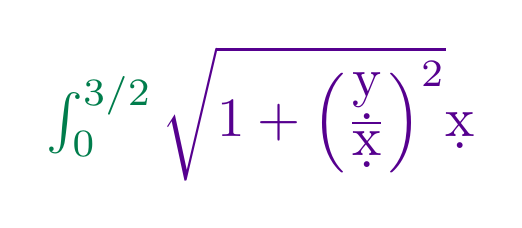
\begin{tikzpicture}[scale=2,every node/.style={transform shape}]
    \node at (0,0) {
      $\color{green!70!black!70!blue}\int_0^{3/2} \color{purple!50!blue!90!black}\sqrt{1 + \left(\frac{\d y}{\d x} \right)^2} \d x$
    };
  \end{tikzpicture}
\end{image}
which can be interpreted conceptually as:
\begin{quote}
  \textbf{The length of a curve is given by the
    \textcolor{green!70!black!70!blue}{accumulated}
    \textcolor{purple!50!blue!90!black}{length determined by the
      instantaneous horizontal change and the instantaneous vertical
      change}.}
\end{quote}
\end{remark}
%%%%%%%%%%%%%%%%%%%%%%%


\section{Length of Curves Formula}
\begin{formula}
Suppose the segment of a curve between the points on $(a,c)$ and $(b,d)$ in the $xy$-plane is defined by a sufficiently differentiable function.  Then, the length of this curve segment is:

\[ s = \int_{x=a}^{x=b} \sqrt{1+\left(\frac{\d y}{\d x} \right)^2} \d x \qquad \qquad \textrm{ or } s = \int_{y=c}^{y=d} \sqrt{1+\left(\frac{\d x}{\d y} \right)^2} \d y \]
\end{formula}



\begin{remark}
Another important point that arises here is that we have complete freedom to express the infinitesimal arclength element $\d s$ in terms of $x$ or $y$.  This will play an important role in the next section. 
\end{remark}

\begin{remark}
For those curious, the phrase ``sufficiently differentiable" here requires that the necessary derivative $\frac{\d y}{\d x}$ or $\frac{\d x}{\d y}$ be piecewise continuous on the interval of integration.
\end{remark}




Let's see a few examples:
\begin{example}%% From guichard
  Find the length of $y = x^{\frac{3}{2}}$ from $x=0$ to $x=2$.
  \begin{explanation}
    Write with me:
    \begin{align*}
      \text{Length} &= \int_0^2 \sqrt{1+\left( \frac{\d y}{ \d x}\right)^2} \d x\\
      &= \int_0^2 \sqrt{1+\left(
        \answer[given]{\frac{3 x^{\frac{1}{2}}}{2}}\right)^2} \d x\\
      &= \int_0^2 \answer[given]{\sqrt{1+\frac{9x}{4}}} \d x
    \end{align*}
      Use the substitution $g = 1+\frac{9x}{4}$ to compute this integral:
      \begin{align*}
	\int_0^2 \sqrt{1+\frac{9x}{4}} \d x &= \frac{4}{9} \int_{\answer[given]{1}}^{\answer[given]{\frac{11}{2}}} g^\frac{1}{2} \d g\\
	&= \frac{4}{9} \left(\frac{2}{3}\right) \eval{g^{\frac{3}{2}}}_{\answer[given]{1}}^{\answer[given]{\frac{11}{2}}}\\
	&=\frac{8}{27} \left(\left(\frac{11}{2}\right)^\frac{3}{2} - 1\right)
      \end{align*}
  \end{explanation}
\end{example}

Just as it was sometimes advantageous to integrate with respect to $y$ in our area and volume calculations, it can also help us sometimes in arclength calculations.  Unlike the area and volume problems, where the geometry of the region often suggested a preferred variable of integration, these problems require us only to consider how we describe the curve in question (and whether we want to work with its given description!) when choosing the variable of integration.
 
\begin{example}
  Find the length of $y = \arcsec(e^x)$ from $x= 0$ to
  $x=\ln(\sqrt{2})$.
  \begin{explanation}
    Trying to write down an integral with respect to $x$ here would be quite annoying.  This problem will be much easier if we work with respect to $y$. Write with me:
    \begin{align*}
      y &= \arcsec(e^x)\\
      \sec(y) &= e^x\\
      \ln(\sec(y)) &= x.
    \end{align*}
    The limits of integration are
    \begin{align*}
      \arcsec(e^0) &= \answer[given]{0}\\
      \arcsec(e^{\ln(\sqrt{2})}) &= \answer[given]{\frac{\pi}{4}}
    \end{align*}
    So now write with me:
    \begin{align*}
      \text{Length} &= \int_0^{\frac{\pi}{4}} \sqrt{1+\left( \answer[given]{\tan(y)} \right)^2} \d y\\
      &=\int_0^{\frac{\pi}{4}} \answer[given]{\sqrt{1+\tan^2(y)}}\d y\\
      &=\int_0^{\frac{\pi}{4}} \answer[given]{\sqrt{\sec^2(y)}}\d y\\
      &=\int_0^{\frac{\pi}{4}} \answer[given]{\sec(y)} \d y\\
      &=\eval{\ln(\sec(x)+\tan(x))}_0^\frac{\pi}{4}\\
      &=\ln(\answer[given]{1+\sqrt{2}}).
    \end{align*}
  \end{explanation}
\end{example}

Sometimes, the integrals that arise can be tricky to compute analytically and require careful differentiation and algebra:

\begin{example}
Find the length of the segment of the curve $y=\frac{1}{3}(2+x^2)^{3/2}$ from $x=0$ to $x=1$.  

\begin{explanation}
We have to differentiate carefully:
\begin{align*}
\ddx\left(\frac{1}{3}(2+x^2)^{3/2}\right) &= \frac{1}{3} \answer[given]{\frac{3}{2}(2+x^2)^{1/2}} \cdot \ddx (\answer[given]{2+x^2}) \\
&= \frac{1}{2} \sqrt{2+x^2} \cdot \answer[given]{2x} \\
&= \answer[given]{x\sqrt{2+x^2}}
\end{align*}

The expression $1+\left(\frac{\d y}{\d x}\right)^2$ in the arclength formula simplifies nicely:
\begin{align*}
1+\left(\frac{\d y}{\d x}\right)^2 &= 1+\left(x\sqrt{2+x^2}\right)^2 \\
&= 1+ \answer[given]{2x^2+x^4} \leftarrow \textrm{ This is a perfect square!} \\
&= \left(\answer[given]{1+x^2}\right)^2
\end{align*}

Thus, the length of the curve segment is:
\begin{align*}
s  = \int_{x=a}^{x=b} \sqrt{1+ \left(\frac{\d y}{\d x}\right)^2} \d x &=  \int_{x=\answer[given]{0}}^{x=\answer[given]{1}} \sqrt{\answer[given]{(1+x^2)^2} }\d x \\
&= \int_{\answer[given]{0}}^{\answer[given]{1}} \answer[given]{1+x^2} \d x \\
&= \eval{\answer[given]{x+\frac{1}{3} x^3}}_{\answer[given]{0}}^{\answer[given]{1}}\\
&= \answer[given]{\frac{4}{3}}
\end{align*}
\end{explanation}
\end{example}

Finally, most of the integrands arising in length calculations do not have elementary antiderivatives, so oftentimes you will only be able to set them up and estimate them numerically.

\begin{example}
  Estimate the length of the curve $y = \sin(x)$ from $x=0$ to $x =  \pi$.  Truncate your answer at the hundredths place.
  \begin{explanation}
    Write with me:
    \begin{align*}
      \text{Length} &= \int_0^\pi \sqrt{1+\left( \frac{\d y}{ \d x}\right)^2} \d x\\
      &= \int_0^\pi \sqrt{1+\left(
        \answer[given]{\cos(x)}\right)^2} \d x
    \end{align*}
    This integral is hard for humans like us, but for our silicon
    friends, it is not so bad.  You can use a computer algebra system
    (or Wolfram Alpha) to approximate this to two decimal places:
    \[
    \text{Length} \approx \answer[given]{3.82}.
    \]
  \end{explanation}
\end{example}

\section{Final thoughts}
To summarize some important points from this section:


\begin{fact}
We have complete freedom to express the infinitesimal arclength element $\d s$ in terms of $x$ or $y$.  Thus, when choosing a variable of integration, consider only whether it would be easier to work with a description of the curve in terms of $x$ or $y$.\end{fact}

\begin{fact}
Most integrals involving radicals are difficult to evaluate and many of the integrands do not have elementary antiderivatives!  Before using numerical software to approximate the integral check whether:

\begin{itemize}
\item The integrand is a square root of a linear function of $x$.  If so, evaluate it by inspection (or by using a substitution if necessary).
\item The expression under the square root is actually a perfect square in disguise.  This often requires careful algebra and differentiation.
\end{itemize}
\end{fact}

As usual, practice is important!  Make sure you work through the problems slowly.  A small mistake early on in the problem can produce catastrophic results.

\begin{quote}
``Did you hear about the mathematician who took up gardening?  He only grows vegetables with square roots!" - Anonymous
\end{quote}


\end{document}
